% P3 -- What confidence actually tracks
\begin{frame}[t]{What confidence actually tracks}{Context volume --- not evidence, not elapsed time}
  \begin{columns}[T]
    \begin{column}{0.48\textwidth}
      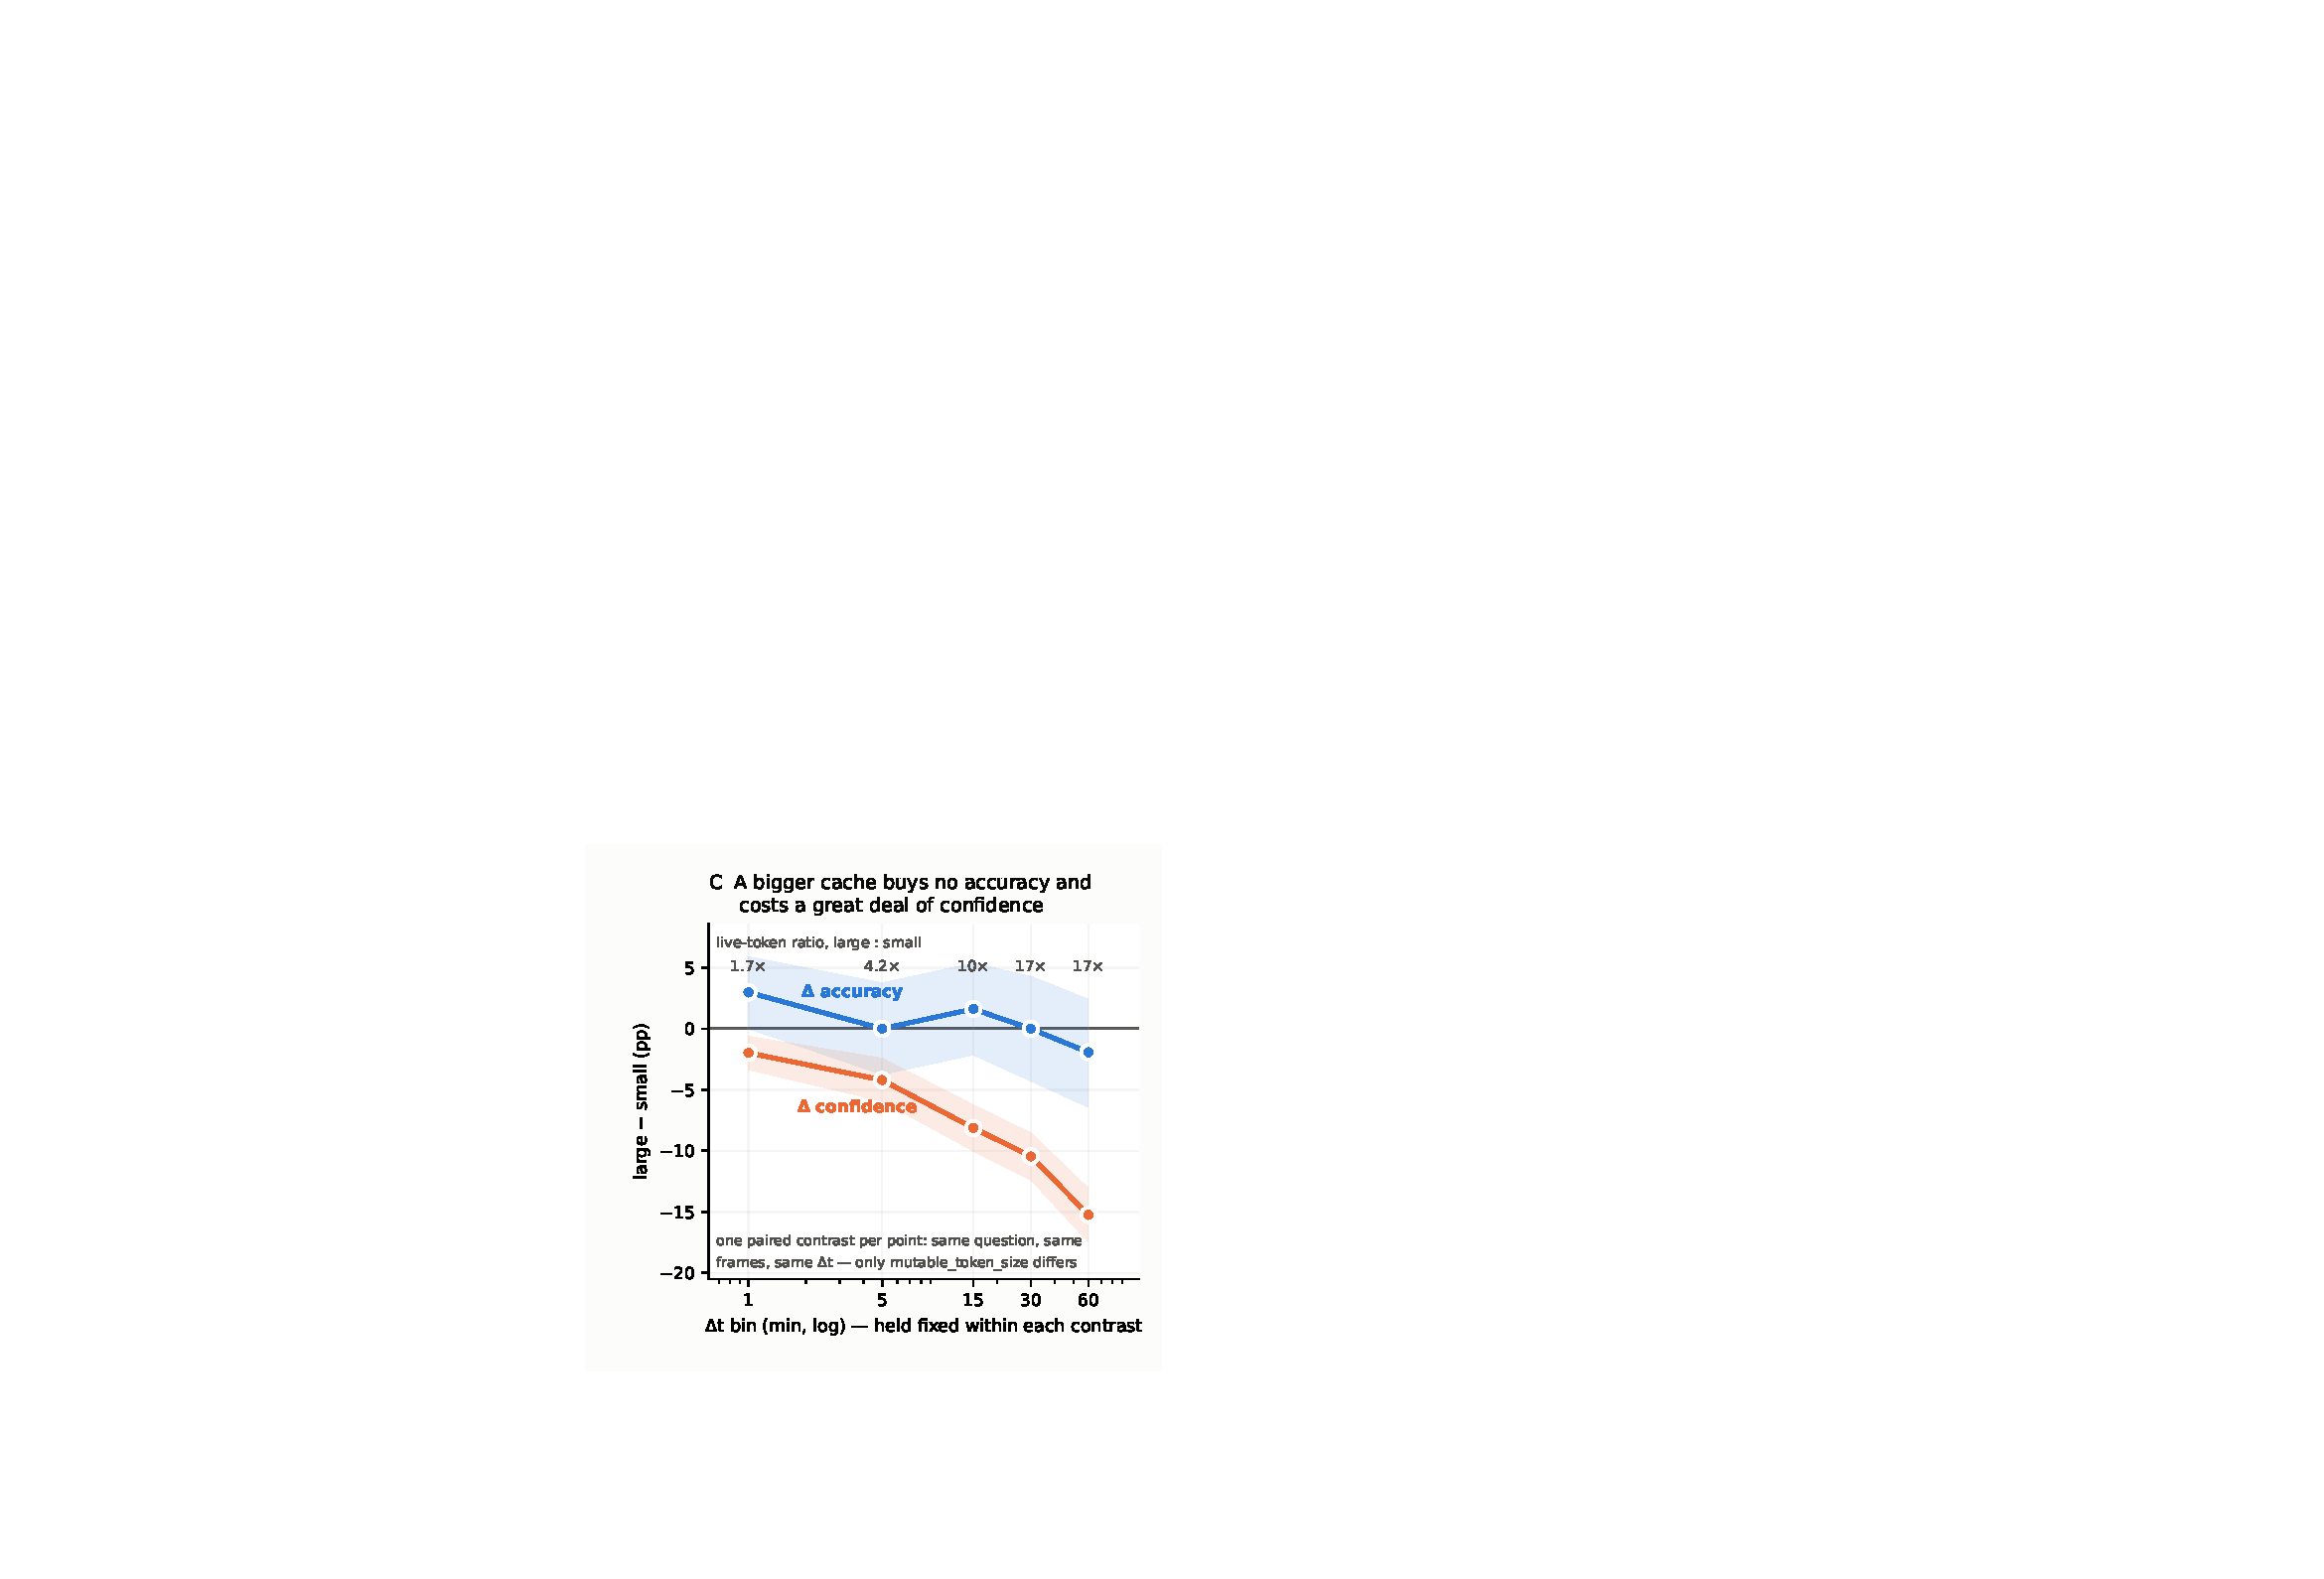
\includegraphics[width=\textwidth,height=0.60\textheight,keepaspectratio]{e2-c.pdf}
      \vskip0.2em
      {\scriptsize\color{inkmid}Budget dose--response (\texttt{large} $-$ \texttt{small}) at each \dt\ bin.}
    \end{column}
    \begin{column}{0.50\textwidth}
      {\footnotesize Varying the memory budget \EtwoBudgetRatio\ at \dt\,=\,60\,min:}
      \vskip0.2em
      \scriptsize
      \begin{tabular}{@{}lr@{}}
        \toprule
        & \thead{$\Delta$ (pp)} \\
        \midrule
        \acc{$\Delta$accuracy} & \EtwoBudgetAcc \\
        \conf{$\Delta$confidence} & \EtwoBudgetConf \\
        \midrule
        \multicolumn{2}{@{}l@{}}{\footnotesize offload-free pair (\CleanBudgetRatio):} \\
        \acc{$\Delta$accuracy} & \emph{\CleanBudgetAcc} \\
        \conf{$\Delta$confidence} & \CleanBudgetConf \\
        \bottomrule
      \end{tabular}
      \vskip0.4em
      {\footnotesize Decomposition of \dt\,=\,15$\rightarrow$60\,min (residual \EtwoDecompResid\ pp):}
      \vskip0.2em
      \scriptsize
      \begin{tabular}{@{}lrr@{}}
        \toprule
        \thead{term} & \thead{\acc{acc}} & \thead{\conf{conf}} \\
        \midrule
        elapsed time & $-$1.68 & \EtwoDecompConfElapsed \\
        context & $-$2.39 & \EtwoDecompConfContext \\
        \bottomrule
      \end{tabular}
    \end{column}
  \end{columns}
  \vskip0.3em
  \claim{\scriptsize More context buys no accuracy and costs a great deal of confidence. The sweep's confidence decline is \textbf{entirely} the context term (\conf{\EtwoDecompConfContext} of \EtwoDecompConfObs\ pp).}
\end{frame}
